\documentclass{article}
\usepackage[utf8]{inputenc}

\usepackage[utf8]{inputenc}
\usepackage[spanish,es-tabla,es-nodecimaldot]{babel}
\usepackage{amsmath,amsthm,amsfonts,amssymb,mathtools,dsfont,mathrsfs}
\usepackage{enumerate,graphicx,xcolor}
\usepackage{lmodern}
\usepackage[T1]{fontenc}
\usepackage[left=2cm,top=2.5cm,right=2cm,bottom=2.5cm]{geometry}
\usepackage[activate={true,nocompatibility},final,tracking=true,kerning=true,spacing=true,factor=1100,stretch=10,shrink=10]{microtype}
\usepackage{hyperref}


%\DeclarePairedDelimiter{\norm}{\lVert}{\rVert}




\newcommand{\N}{\mathbb{N}}
\newcommand{\R}{\mathbb R}
\newcommand{\Z}{\mathbb Z}
\newcommand{\Rbar}{\overline{\mathbb R}}
\newcommand{\F}{\mathscr F}
\newcommand{\A}{\mathscr A}
\newcommand{\To}{\Rightarrow}
\newcommand{\C}{\mathscr C}
\newcommand{\La}{\mathscr L_A}
\newcommand{\B}{\mathcal B}
\newcommand{\Q}{\mathbb Q}
\renewcommand{\epsilon}{\varepsilon}
\renewcommand{\L}{\mathcal L}
\renewcommand{\d}{\mathrm d}
\newcommand{\abs}[1]{\left| #1 \right|}
\newcommand{\pts}[1]{\left( #1 \right)}
\newcommand{\norm}[1]{\left\lVert#1\right\rVert}
\renewcommand{\P}[1]{\mathbb P\left( #1 \right)}
\newcommand{\E}[1]{\mathbb E \left( #1 \right)}


\newcommand{\ols}[1]{\mskip.5\thinmuskip\overline{\mskip-.5\thinmuskip {#1} \mskip-.5\thinmuskip}\mskip.5\thinmuskip} % overline short
\newcommand{\olsi}[1]{\,\overline{\!{#1}}} % overline short italic
\makeatletter
\newcommand\closure[1]{
  \tctestifnum{\count@stringtoks{#1}>1} %checks if number of chars in arg > 1 (including '\')
  {\ols{#1}} %if arg is longer than just one char, e.g. \mathbb{Q}, \mathbb{F},...
  {\olsi{#1}} %if arg is just one char, e.g. K, L,...
}
% FROM TOKCYCLE:
\long\def\count@stringtoks#1{\tc@earg\count@toks{\string#1}}
\long\def\count@toks#1{\the\numexpr-1\count@@toks#1.\tc@endcnt}
\long\def\count@@toks#1#2\tc@endcnt{+1\tc@ifempty{#2}{\relax}{\count@@toks#2\tc@endcnt}}
\def\tc@ifempty#1{\tc@testxifx{\expandafter\relax\detokenize{#1}\relax}}
\long\def\tc@earg#1#2{\expandafter#1\expandafter{#2}}
\long\def\tctestifnum#1{\tctestifcon{\ifnum#1\relax}}
\long\def\tctestifcon#1{#1\expandafter\tc@exfirst\else\expandafter\tc@exsecond\fi}
\long\def\tc@testxifx{\tc@earg\tctestifx}
\long\def\tctestifx#1{\tctestifcon{\ifx#1}}
\long\def\tc@exfirst#1#2{#1}
\long\def\tc@exsecond#1#2{#2}
\makeatother

\newtheorem{lemma}{Lema}
\newtheorem{theorem}{Teorema}

\setlength\parindent{0pt}
\setlength\parskip{4pt}


\title{Cómputo científico para probabilidad y estadística. Tarea 9.\\
MCMC: Tarea Final}
\author{Juan Esaul González Rangel}
\date{Diciembre 2023}



\begin{document}

\maketitle

En ambos problemas hay que diseñar e implementar el MCMC, investigar sobre su 
convergencia y tener algún grado de certeza sobre si sí se está simulando de la 
posterior correspondiente. Más aún, recuerde que se trata de un problema de 
inferencia: Hay que hablar del problema en sí, comentar sobre las posteriores 
simuladas y posibles estimadores (a partir de la muestra de posterior) que se 
pueden proporcionar de cada parámetro.

\begin{enumerate}
    \item (\textbf{Problema en ecología}) Sean $X_1, \dots, X_m$ variables aleatorias 
    donde $X_i$ denota el número de individuos de una especie en cierta región. 
    Suponga que $X_i|N, p \sim $Binomial$(N, p)$, entonces
    
    \[f (\bar x|N, p) = \prod_{i=1}^m \frac{N!}{x_i!(N - x_i)!}p^{x_i} 
    (1 - p)^{N - x_i}.\]

    Asumiendo la distribución a priori $p \sim $Beta$(\alpha, \beta)$ y 
    $N \sim h(\cdot)$, donde $h$ es una dist. discreta en $\{0, 1, 2, \dots , 
    N_{\max} \}$, se tiene definida la distribución posterior $f (N, p |\bar x)$.
    
    A partir del algoritmo MH, simule valores de la distribución posterior usando un 
    kernel híbrido. Para ello considere como sugerencia la siguiente distribución 
    inicial para el MCMC 
    
    \[p \sim U(0, 1) \text{ y } N \sim U_d \left\{\max_{i\in\{1,\dots,m\}}(x_i), 
    \max_{i\in\{1,\dots,m\}}(x_i) + 1, \dots , N_{\max}\right\}\]
    
    y las propuestas

    \begin{itemize}
        \item Propuesta 1: De la condicional total de p (kernel Gibbs).
        \item Propuesta 2: De la a priori.
        \item Propuesta 3: Propuesta hipergeométrica (¿?).
        \item Propuesta 4: Poisson: $N_p \sim \max_{i\in\{1,dots,m\}}(x_i) + 
        $Poisson(?).
        \item Propuesta 5: Caminata aleatoria
    
    \[N_p = N + \epsilon, \qquad P(\epsilon = 1) = \frac12 = P(\epsilon = -1).\]
    
    Los datos son estos: 7, 7, 8, 8, 9, 4, 7, 5, 5, 6, 9, 8, 11, 7, 5, 5, 7, 3, 10, 3.
    
    A priori, esperamos que sea difícil observar a los individuos entonces $\alpha = 1, \beta = 20$. La especie no es muy abundante y entonces $N_{\max} = 1000$ y $h(N ) = 1/(N_{\max} + 1); N \in \{0, 1, 2, . . . , N_{\max}\}$.

    Las propuestas y distribución inicial para el MCMC de arriba son \textbf{solamente sugerencia}, propongan otras propuestas, experimenten y comenten.
    \end{itemize}


    \begin{proof}[Solución]
        La forma en que se resolvieron las distintas propuestas es la siguiente:

        \begin{itemize}
            \item Para encontrar el kernel de Gibbs para $p$ multiplicamos la 
            verosimilitud por la densidad a priori de $p$, al tratarse de una binomial 
            y una beta, sabemos que es una familia conjugada, y podemos encontrar a la
            posterior como una distribución Beta$\left(\alpha + \sum_{i=1}^m x_i,
            \beta + \sum_{i=1}^m (N-x_i) \right)$.
            
            \item La distribución a priori para $p$ es Beta$(\alpha,\beta)$, y para 
            $N$ es $U_d\left\{0,1,\dots,N_{\max}-1,N_{\max}\right\}$, como no hay 
            dependencia entre ellas podemos suponerlas independientes y la densidad 
            conjunta es el producto de las densidades.

            \item Para la hipergeométrica se usó como la cantidad de elementos totales 
            el número $N_{\max}$, como cantidad de elementos del tipo que nos interesan el
            número $N_t$ (la $t$-ésima iteración de la cadena), y como tamaño de la muestra
            que se revisa se experimentó con varias cantidades y al final con 500 se obtuvo 
            el mejor desempeño.

            \item Para la distribución Poisson se experimentó con varias propuestas de tasa,
            incluyendo algunas que toman en cuenta el valor actual de $p$ o de $N$ y el número
            $N_{\max}$, pero al final se observó un mejor comportamiento usando como tasa
            simplemente el valor actual de $N$.

            \item En la propuesta 5 no había ninguna decisión que tomar, pero tanto en esta 
            como en las propuestas anteriores, había que tomar en cuenta que si un valor 
            propuesto de $N$ se sale del rango $\{0,\dots,N_{\max}\}$, se rechaza 
            inmediatamente.

            \item Adicionalmente, se experimentó agregando otras dsitribuciones discretas 
            para $N$ y continuas en $(0,1)$ para $p$, la que mejor funcionó fue la distribución
            binomial$(N_{\max},p)$ para $N$, pero esta tendía a proponer valores muy centrales,
            lo que ocasionaba que el algoritmo recorriera el soporte más lentamente, así que se
            le agregó una probabilidad menor de ocurrencia que a las otras propuestas.
        \end{itemize}

        Al usar un kernel híbrido, sabemos que se cumple balance detallado, y junto con la 
        irreducibilidad proporcionada por las propuestas con soporte en todos los valores
        de interés, tenemos que lo único necesario para la convergencia es la aperiodicidad
        fuerte, pero esta está garantizada por el hecho de que varias propuestas tienen 
        probabilidad positiva de rechazar la transición.

        Al hacer 10,000 iteraciones de este algoritmo de MCMC, tenemos las siguientes
        trayectorias para la evolución de $p$ y de $N$,

        \begin{center}
            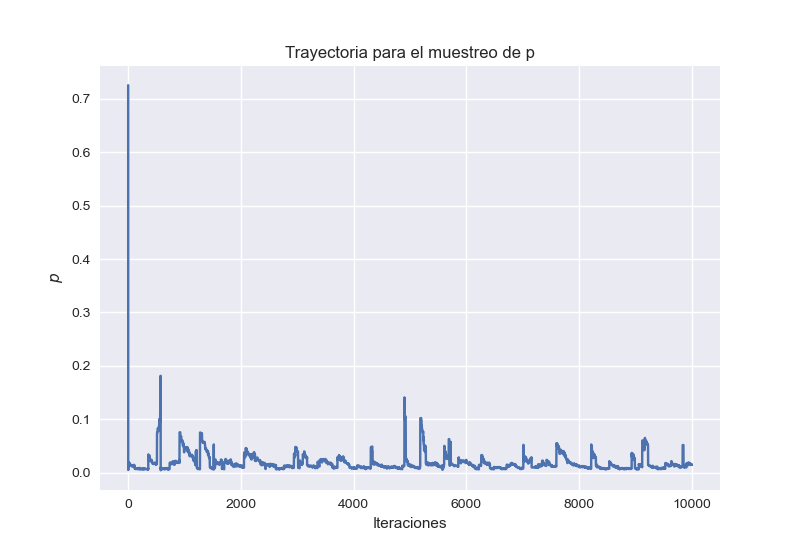
\includegraphics[width=0.8\textwidth]{Tarea9/trajp.png}
            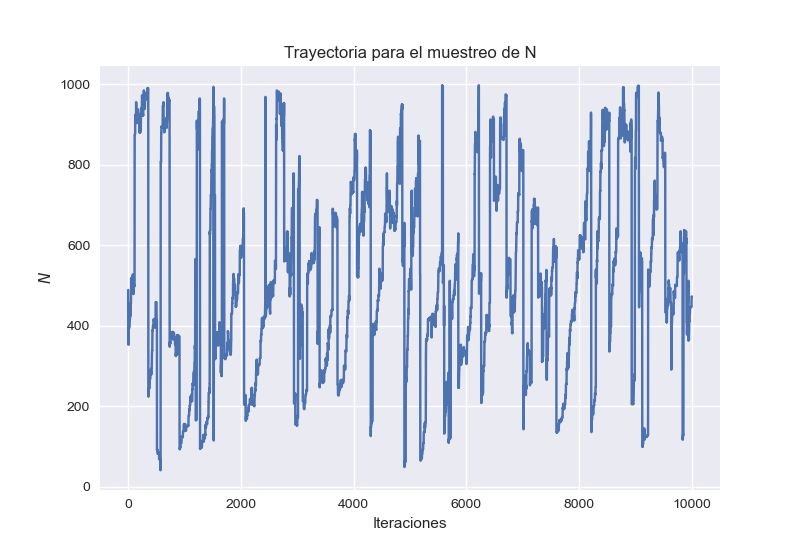
\includegraphics[width=0.8\textwidth]{Tarea9/trajN.png}
        \end{center}

        Notemos que la trayectoria de $p$ tiende a estabilizarse pronto en valores cercanos 
        a cero, a pesar de que la distribución inicial es uniforme en $(0,1)$, mientras que 
        la trayectoria de $N$ se mueve más a lo largo de todo el dominio, aunque toma valores
        centrales más frecuentemente.

        En la siguiente figura se observa el comportamiento de la trayectoria en coordenadas
        $p$ y $N$ de la cadena,

        \begin{center}
            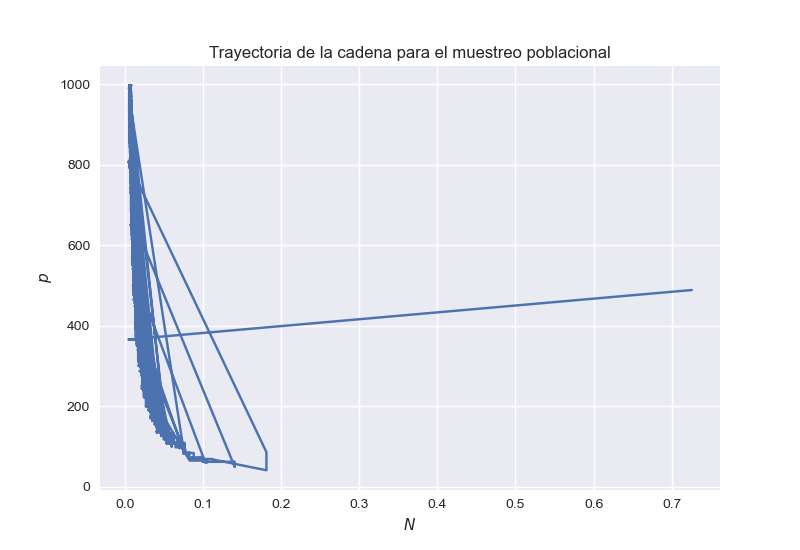
\includegraphics[width=0.8\textwidth]{Tarea9/trajpN.png}
        \end{center}

        En la trayectoria podemos observar un dominio de atracción, que corresponde a 
        los puntos en donde se concentra más la masa de la distribución, y que se localiza
        hacia el extremo inferior del soporte en $p$.

        En el contexto del número de individuos, la posterior nos dice que las probabilidades
        de observación son bajas, aun cuando se suponga que hay abundancia de la especie.

        Para saber si la simulación corresponde realmente a la distribución que nos interesa,
        podemos graficar el logaritmo de la densidad evaluada en la cadena contra las
        iteraciones, obteniendo la gráfica de burn-in que se muestra a continuación,

        \begin{center}
            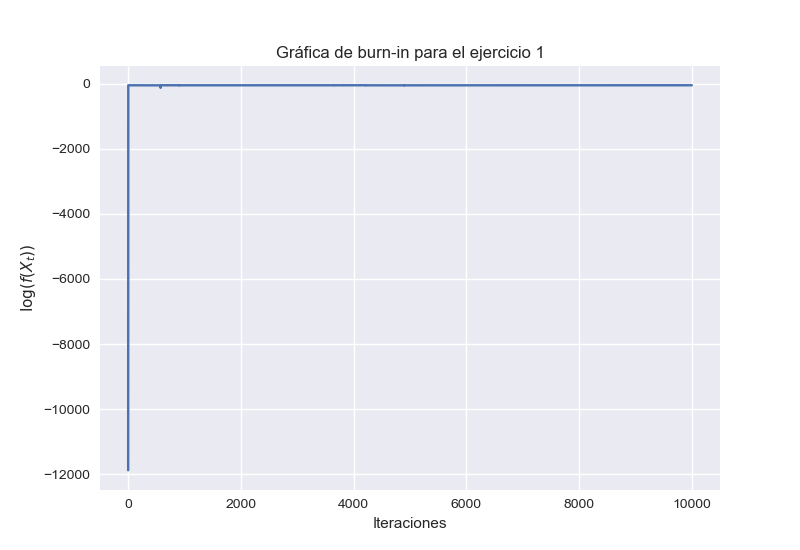
\includegraphics[width=0.68\textwidth]{Tarea9/burnin1.png}
        \end{center}

        La gráfica muestra un comprtamiento muy irregular, con unos primeros puntos que 
        distan mucho del comportamiento a largo plazo de la cadena, por lo que podemos decir
        que estos es posible descartar estas primeras observaciones para obtener información
        más útil sobre $N$ $p$. Al descartar los primeros 100 valores muestreados, obtenemos
        los siguientes histogramas para $N$ y $p$,

        \begin{center}
            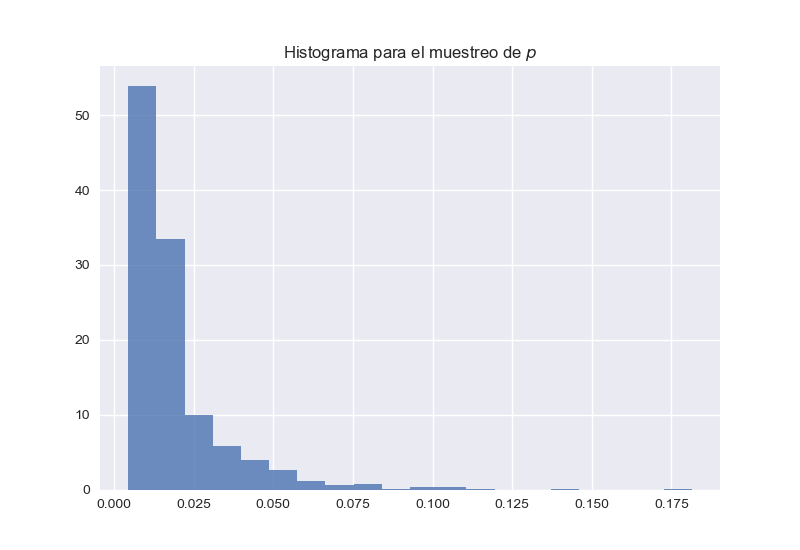
\includegraphics[width=0.68\textwidth]{Tarea9/histp.png}
            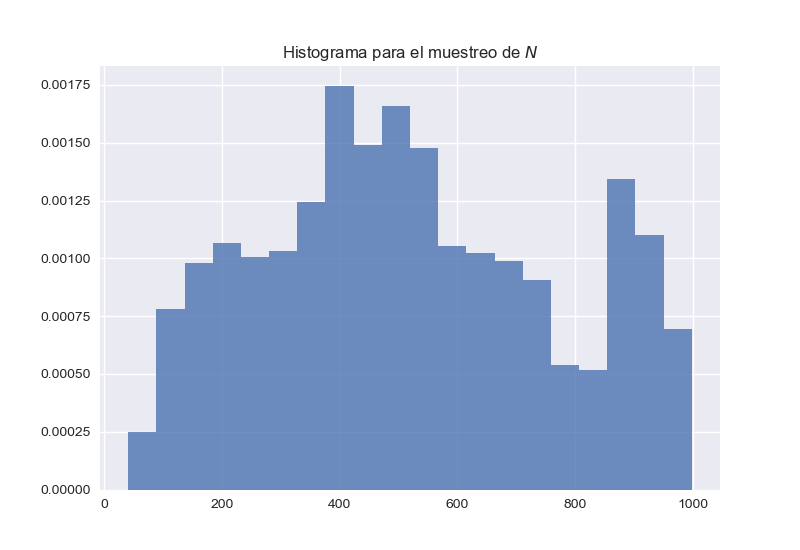
\includegraphics[width=0.68\textwidth]{Tarea9/histN.png}
        \end{center}

        El histograma de $N$ parece ser bimodal, lo que podría indicar que hay menos certidumbre
        sobre el valor de este parámetro. El valor de $p$, en cambio, se concentra muy claramente
        entre 0 y 0.025, por lo que hay más certeza sobre su valor.

        Un estimador de interés que se puede obtener a partir de estas simulaciones es
        el producto de las medias muestrales de $N$ y $p$ como estimador de la esperanza
        de $X_i$. Estos estimadores son $\bar p = 0.01868$ y $\bar N = 517.819$, por lo que
        el estimador encontrado de esta forma es $\widehat{ \E{X_i} } = 9.6746$.

        En función del tipo de estimador que se busque y de las propiedades que se espera
        que cumpla, es posible obtener de la muestra otras características, como desviación
        típica de los parámetros, medianas como estimadores robustos o cuantiles para estimar
        las probabilidades de encontrar una cantidad atípica de individuos.




    \end{proof}


    \item (\textbf{Estudio de mercado}) Se tiene un producto y se realiza una encuesta con el fin de estudiar cuánto se consume dependiendo de la edad. Sea $Y_i$ el monto de compra y $X_i$ la covariable la cual representa la edad.
    
    Suponga que $Y_i \sim Po(\lambda_i)$ (distribución Poisson con intensidad $\lambda_i$)
    
    \[\lambda_i = cg_b(x_i - a)\]

    para $g_b$ la siguiente función de liga 
    
    \[ g_b(x) = \exp\left(- \frac{x^2}{2b^2}\right) .\]

    O sea, se trata de regresión Poisson con una función liga no usual. Si $\lambda_i = 0$ entonces $P(Y_i = 0) = 1$. $a = $años medio del segmento (años), $c = $gasto promedio (pesos), $b = $``amplitud'' del segmento (años).

    Considere las distribuciones a priori
    
    \[a \sim N (35, 5), \qquad c \sim Gama(3, 3/950), \qquad b \sim Gama(2, 2/5).\]
    
    El segundo parámetro de la normal es desviación estandard y el segundo parámetro de las gammas es taza (rate).
    
    Usando MH simule de la distribución posterior de a, c y b.
    
    Los datos son estos, n = 100:

\begin{verbatim}
X = array([ 25, 18, 19, 51, 16, 59, 16, 54, 52, 16, 31, 31, 54, 26, 19, 13, 59, 48, 54, 23, 50, 59, 
55, 37, 61, 53, 56, 31, 34, 15, 41, 14, 13, 13, 32, 46, 17, 52, 54, 25, 61, 15, 53, 39, 33, 52, 65, 
35, 65, 26, 54, 16, 47, 14, 42, 47, 48, 25, 15, 46, 31, 50, 42, 23, 17, 47, 32, 65, 45, 28, 12, 22, 
30, 36, 33, 16, 39, 50, 13, 23, 50, 34, 19, 46, 43, 56, 52,42, 48, 55, 37, 21, 45, 64, 53, 16, 62, 
16, 25, 62])

Y = array([1275, 325, 517, 0, 86, 0, 101, 0, 0, 89, 78, 83, 0, 1074, 508, 5, 0, 0, 0, 1447, 0, 0, 
0, 0, 0, 0, 0, 87, 7, 37, 0, 15, 5, 6, 35, 0, 158, 0, 0, 1349, 0, 35, 0, 0, 12, 0, 0, 2, 0, 1117, 0, 
79, 0, 13, 0, 0, 0, 1334, 56, 0, 81, 0, 0, 1480, 177, 0, 29, 0, 0, 551, 0, 1338, 196, 0, 9, 104, 0, 
0, 3, 1430, 0, 2, 492, 0, 0, 0, 0, 0, 0, 0, 0, 1057, 0, 0, 0, 68, 0, 87, 1362, 0]) \end{verbatim}


    \begin{proof}[Solución]
        Los tres parámetros dependen de $X$ y $Y$ a través de las tasas $\lambda_i$ y la
        verosimilitud evaluada en $Y$. Como existen relaciones entre $a,b$ y $c$, es necesario
        que se muestree de ellos usandolos como un vector aleatorio $(a,b,c)$, en lugar de
        como marginales. 

        El algoritmo diseñoado consiste en tres kerneles distintos que simulan cada uno de
        una de las variables, esto podría causar que la convergencia sea más lenta, pero nos
        facilita la decisión de las propuestas de transición, pues únicamente necesitamos
        que la transición sea aceptada en una dirección. La elección de las propuestas fue 
        con base en ensayo y error, y considerando que los parámetros represetan cantidades
        cuoys valores están restringidas a un cierto dominio. 
        
        Para la edad se 
        necesitaba que siempre fueran positiva, así que se propuso una transción gamma, en el caso
        de la amplitud del segmento, también se necesitaba una cantidad no negativa pues 
        representa una cantidad en años, así que se usó otra gamma, pero se cambiaron el punto
        inicial y los parámetros para que ambas muestrearan el espacio en rangos de valores
        adecuados de acuerdo con su escala.

        Para el gasto promedio se usó una caminata aleatoria, y se localizó con un valor inicial
        cerca de 5000, pues este tendía a ser atractivo para la cadena cuando se inicializaba 
        en otros puntos.

        Se simularon 10,000 puntos de la posterior conjunta
        las trayectorias de las cadenas marginales se muestran a continuación,

        \begin{center}
            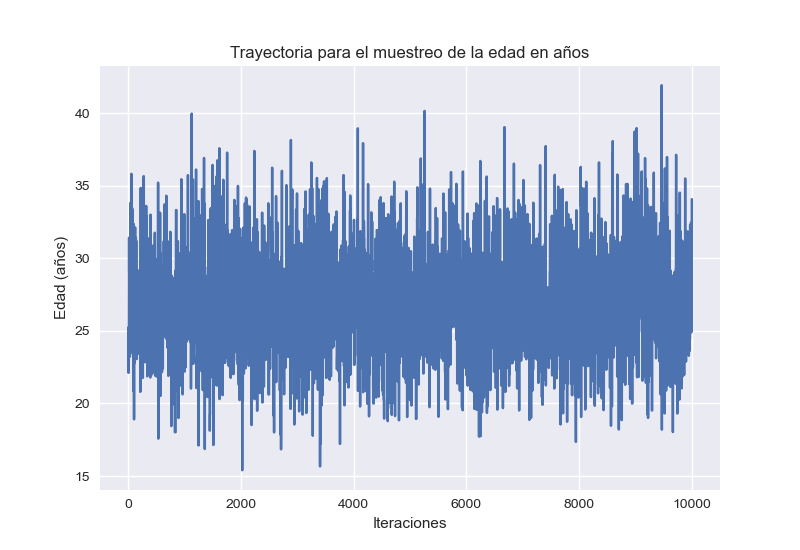
\includegraphics[width=0.8\textwidth]{Tarea9/traja.png}
            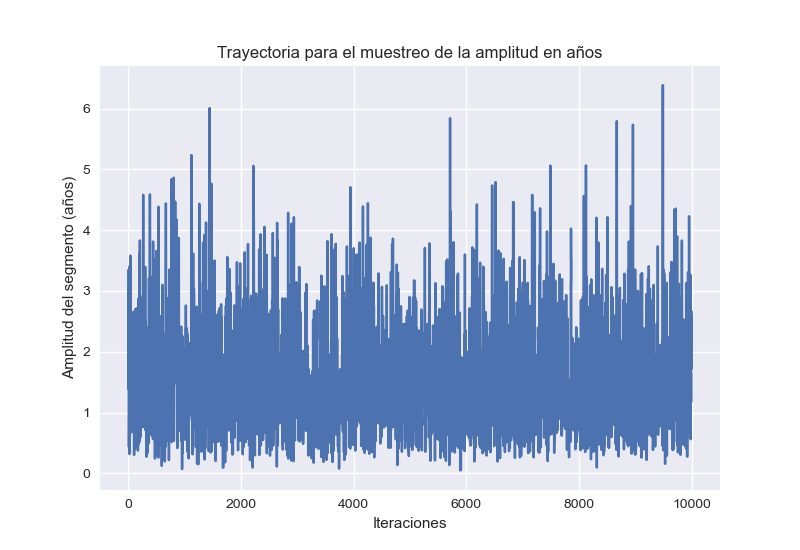
\includegraphics[width=0.8\textwidth]{Tarea9/trajb.png}
            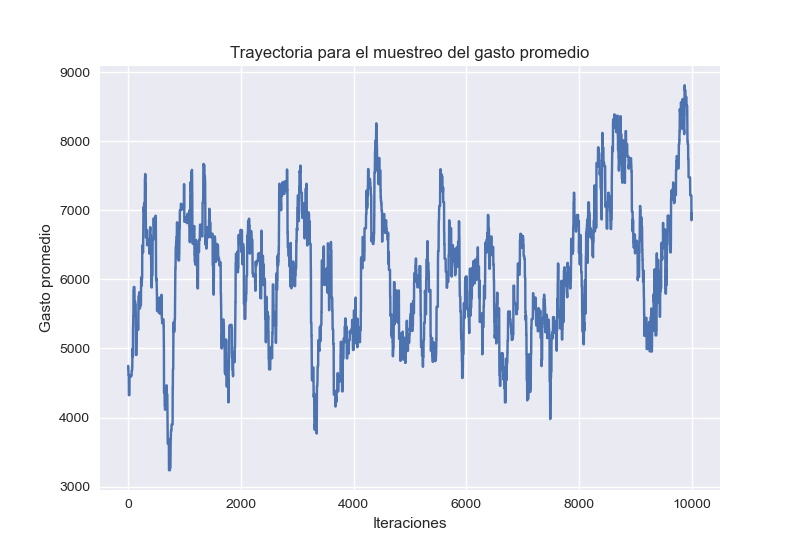
\includegraphics[width=0.8\textwidth]{Tarea9/trajc.png}
        \end{center}

        Notemos que el rango de los valores de la edad se encuentra entre 15 y 40, 
        lo que concuerda con los datos observados $X_i$, mientras que el rango de
        los montos de compra simulados está entre 3,000 y 9,000, contrastando con los
        valores observados $Y_i$. La discrepancia en el último grupo de valores podría
        deberse a que las distribuciones a priori consideradas no son no informativas, 
        lo que podría modificar las conclusiones creadas a partir de los datos.

        Los histogramas de los tres parámetros aparecen a continuación,

        \begin{center}
            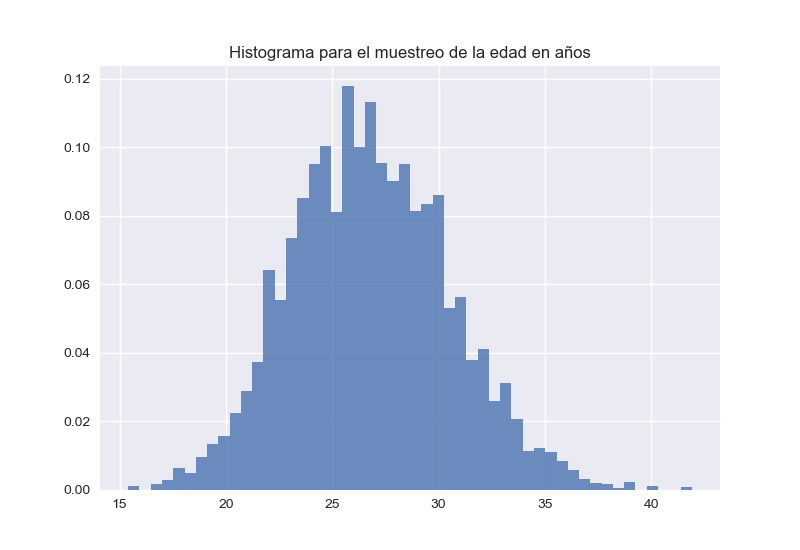
\includegraphics[width=0.75\textwidth]{Tarea9/hista.png}
            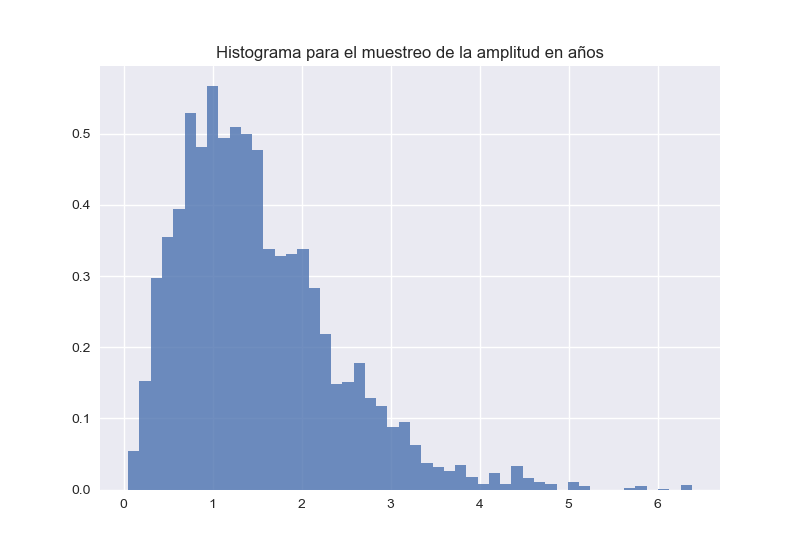
\includegraphics[width=0.75\textwidth]{Tarea9/histb.png}
            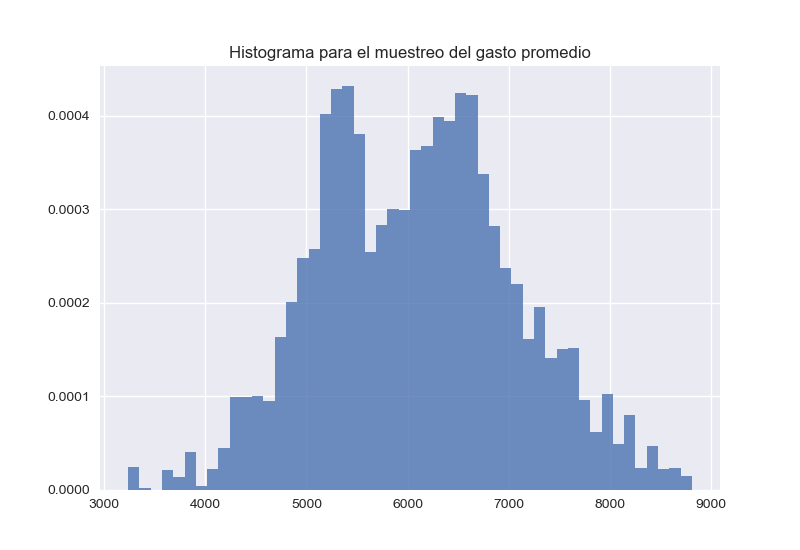
\includegraphics[width=0.75\textwidth]{Tarea9/histc.png}
        \end{center}

        Notamos que el parámetro edad muestra un comportamiento similar a una normal
        con media 27, mientras que el gasto promedio tiene distribución bimodal y se 
        encuentra ubicado alrededor de 6000. La amplitud del segmento se concentra 
        alrededor de 1 año, y es no negativa, con algunos valores atípicos a la derecha.

        Las medias de las posteriores encontradas son las siguientes

        \begin{center}
            \begin{tabular}{cl}
                \hline
                \multicolumn{1}{l}{Parámetro} & Media \\ \hline
                a & 26.811 \\
                b & 1.5109 \\
                c & 6095.27 \\ \hline
                \end{tabular}
        \end{center}

        Tomando en cuenta los datos proporcionados, las edades parecen ajustar bien
        la distribución de la que provienen los datos $X_i$ observados, mietras que los
        gastos promedio difieren bastante, lo que hace suponer un error numérico o una
        mala previa para la distribución del parámetro $c$.


    \end{proof}

    \item Investiga y describe muy brevemente los softwares OpenBugs, Nimble, 
    JAGS, DRAM, Rtwalk, Mcee Hammer, PyMCMC.

    En la página oficial de OpenBUGS se menciona que es un programa de código 
    abierto para la modelación Bayesiana desarrollado sobre WinBUGS. Se menciona
    tabién que el desarrollo de OpenBUGS ya no está activo y actualmente BUGS se
    enfoca en mantener el software MultiBUGS. Más concretamente, en 
    \textit{The BUGS project: Evolution, critique and future directions} se indica 
    que el proyecto BUGS (Bayesian inference Using Gibbs Sampling) surge en la 
    unidad de bioestadística del consejo de investigación médica de la Universidad
    de Cambridge en 1989.  
    
    Fundamentalmente, OpenBUGS (o WinBUGS o MultiBUGS) se basa en la modelación 
    gráfica de las dependencias entre parámetros. Mediante una gráfica dirigida
    acícilca (DAP) se puede expresar cuáles son los componentes del modelo y cómo
    se relacionan entre ellos, mediante dependencias estocásticas y funcionales.
    Las ventajas de utilizar esta representación de los modelos en OpenBUGS es que
    se permite expresar relaciones de manera sencilla mediante el lenguaje propio que
    incorpora el software, y que el tener la gráfica de relaciones permite que
    WinBUGS sepa exactamente qué cálculos son los mínimos que se necesitan realizar
    para encontrar un condicionamiento total, logrando de esta manera ahorrar recursos
    como tiempo o almacenamiento.

    Los softwares de BUGS son bastante populares, y esta popularidad se debe a que
    son muy flexibles y por lo tanto resultan útiles en una gran diversidad de 
    contextos. La desventaja de la flexibilidad que presenta OpenBUGS es que al
    ser usado en tantas situaciones distintas, pueden aparecer nuevos problemas
    derivados de casos específicos de aplicación quen no se habían considerado
    previamente.

    Según su página oficial, Nimble es una adopción de OpenBUGS a R que permite
    manipular modelos y objetos para usarlos dentro de R, a comparación de otras
    interfaces de OpenBUGS para R que únicamente permiten usar simulaciones MCMC
    dentro de R. Entre las ventajas que Nimble provee están el permitir distantas 
    parametrizaciones de las distribuciones y usar distribuciones definidas por
    el usuario.

    JAGS son las siglas de Just Another Gibbs Sampler y puede entenderse como una
    variación de BUGS creada con el propósito de ser multiplataforma, compatible
    con BUGS, ser extensible permitiendo a los usuarios escribir sus propias 
    funciones, distribuciones y simuladores.

    Las siglas de DRAM son Delaying Rejection Adaptive Metropolis, y como su nombre
    lo indica, es la mezcla de dos técnicas recientes para la mejora de algoritmos
    MCMC, el primero llamado Metropolis Adaptativo mejora la eficiencia de convergencia 
    y el segundo, Rechazo retardado ayuda a resolver situaciones en las que el 
    Metropolis Adaptativo tiene problemas para empezar. En conjunto, los algoritmos
    logran mejores resultados que implementaciones tradicionales, aunque su eficiencia
    siempre depende de las distribuciones de las que se intenta simular y por lo tanto
    no es mejor en todas las situaciones.

    El software t-walk en general es algoritmo de propósito general para muestrear
    de distribuciones conjuntas. En su página oficial se afirma que sirve para muestrear
    de una gran variedad de distribuciones, por lo que es especialmente útil para
    simular posteriores en estadística Bayesiana o en otros contextos en los que sea
    difícil usar software tradicional. El t-walk no necesita refinamiento por parte
    del usuario
    Como consecuencia de esta flexibilidad, el t-walk puede tener un desempeño peor 
    que los programas diseñados para muestrear especificamente de una distribución 
    en particular, aunque su propósito es ser generalista. Rtwalk es la implementación
    en R de t-walk.

    El algoritmo emcee Hammer es una implementación pura en Python de un método MCMC para 
    muestreo que es invariante para transformaciones afines. El hecho de que el método
    sea invariante bajo transformaciones afines hace que result muy útil cuando
    se trabaja con una dsitribución mal escalada, mientras que el hecho de que el
    algoritmo esté implementado en Python lo hace accesible a muchas personas, al ser
    el lenguaje de programación más usado actualmente.

    Al igual que emcee Hammer, PyMCMC es una implementación de un algoritmo MCMC en 
    Python, logrando con esto la ventaja de estar disponible en un leguaje con sintaxis
    sencilla y una gran cantidad de usuarios. Además de los métodos MCMC, PyMCMC también
    provee con otras herramientas estadísticas como algoritmos de inferencia variacional.
    Una de las principales ventajas de PyMCMC es que usa un paradigma llamado programación
    probabilística, lo que le permite que el usuario defina modelos directamente 
    en sintaxis de Python sin necesidad de usar un leguaje ajeno.


   
\end{enumerate}




 \end{document}